\chapter{Implementation}
\label{sec:implementation}

This project is implemented in Python, making use of the Django web framework
and the Twisted networking engine.

\section{Python}
\label{sec:implementation-python}

\begin{figure}[h]
    \footnotesize
    \begin{verbatim}
    Beautiful is better than ugly.
    Explicit is better than implicit.
    Simple is better than complex.
    Complex is better than complicated.
    Flat is better than nested.
    Sparse is better than dense.
    Readability counts.
    Special cases aren't special enough to break the rules.
    Although practicality beats purity.
    Errors should never pass silently.
    Unless explicitly silenced.
    In the face of ambiguity, refuse the temptation to guess.
    There should be one-- and preferably only one --obvious way to do it.
    Although that way may not be obvious at first unless you're Dutch.
    Now is better than never.
    Although never is often better than *right* now.
    If the implementation is hard to explain, it's a bad idea.
    If the implementation is easy to explain, it may be a good idea.
    Namespaces are one honking great idea -- let's do more of those!
    \end{verbatim}
    \caption{The Zen of Python, by Tim Peters}
    \label{fig:zen-of-python}
\end{figure}

The backup system is implemented in Python, which is a fast, powerful and
dynamic programming language, suitable for a large variety of application
domains \cite{sanner1999}.

Python has a large and feature-rich standard library, and also has many
frameworks and third-party libraries available. Its clean, concise and readable
syntax also make it a pleasant programming language to work with.

Python was created by Guido van Rossum in the early 1990s. To ensure a clear,
easy-to-use language, van Rossum only used ideas that had proven their worth
over time in other programming languages. In particular, he wanted a language
that would be easy to extend for use with other languages \cite{lindstrom2005}.

Traditionally, systems of this nature would most likely be implemented in
a more ``classic'' language such as C or C++. Python offers a modern
alternative to these---not only in syntax but also in mindset.

So-called Python ``extension libraries'' can be written in C or C++, providing
low-level, fast access to the internal Python language. This makes Python
particularly suitable for use with this project, as proof-of-concept code can
be written in Python for ease---and then rewritten in C or C++ later if
performance is found to be an issue.

Python is modular by nature, allowing the core language kernel to be extended
by importing any number of extension modules (or \emph{packages}). The Python
distribution includes a diverse library of standard extensions (some written in
Python itself, others in C or C++).

\subsection{Python Packages}

Python packages can be installed in myriad different ways. Firstly, a properly
packaged Python module will always contain a file \verb!setup.py! in the root
directory, which can be used to install the package by running it from the
command line: \verb!python setup.py install!. This process will place the
required files in the correct location(s) on the file system, so they can be
imported properly by the Python interpreter. Also, if any extensions require
compilation (i.e. C or C++ code) this will be done automatically.

Python has a central repository for packages---the Python Package Index (PyPI
for short, also known as ``The Cheese Shop'', in reference to a 1972 sketch by
Monty Python)---which can be used to download and install extension modules
automatically.

Packages located on PyPI can be acquired using a tool called \emph{pip}, which
takes care of downloading and installing the required package, along with all
of its dependencies. This is by far the fastest and most convenient way of
installing Python packages.

\subsection{virtualenv and virtualenvwrapper}

\emph{virtualenv} is a Python tool which allows developers to create multiple,
isolated Python environments on the same computer. This has many advantages,
including the ability to maintain different versions of the same package or
framework, and to install or upgrade packages without the need for
root/administrator access.

To use a virtual environment, it must first by ``activated''. This process
simply consists of \emph{sourcing} a script which modifies the
\verb!$PYTHONPATH! environment variable, allowing the Python interpreter to
import packages from the correct location.

\emph{virtualenvwrapper}, as the name suggests, is a wrapper program for
virtualenv. It augments the functionality to make creating, activating and
deleting virtual environments easier. It also ensures that commonly used
packages (such as \emph{pip}) are installed in new virtual environments by
default.

\section{Django}
\label{sec:implementation-django}

The system implementation is based on top of the Django framework which, though
primarily designed for creating web applications, can be used as the basis for
any type of application.

\begin{quote}
    \emph{Django is a high-level Python Web framework that encourages rapid
    development and clean, pragmatic design.}\footnote{www.djangoproject.com}
\end{quote}

\subsection{MVC}

Django uses the Model-View-Controller (MVC) design pattern. The key idea in the
MVC pattern is to separate the user interface from the underlying data
represented by that interface. In MVC, the View displays information to the
user and, combined with the Controller which processes the user's interaction,
comprises the application's user interface. The Model contains both the data
represented by the View, and logic that changes this data in response to user
interaction \cite{leff2001}.

Use of the MVC pattern makes development and maintenance of applications easier
for a number of reasons. For example, the application's appearance can be
drastically changed without altering the underlying data structures or business
logic. Also, the application can have different ``interfaces'', providing
access to the same data in a multitude of ways (i.e. in different languages, or
data formats) \cite{leff2001}.

\subsection{Reusable Apps}

Perhaps the most appealing aspect of Django is that of \emph{reusable apps}.
Django's architecture not only separates the Models, Views, and Controllers
(i.e. the MVC pattern) but also encourages developers to separate the
functionality of the overall system into loosely-coupled \emph{apps}. An app
defines its own Models, View and Templates (Django's terminology slightly
differs from standard MVC frameworks by referring to Controllers as ``Views''
and Views as ``Templates''). These apps can then be packaged up as Python
modules, and published for the community on the Python Package Index.

As an example, an app providing user registration with e-mail validation is
available, and commonly used in systems which require this functionality.

In this project, Django is used to provide access to the database (the
\emph{models}) and for the web interface itself. The only 3\textsuperscript{rd}
party app used in the backup system is called \emph{haystack}, which provides
a simple Django-like API for searching the data models. This is discussed in
more detail in section \ref{sec:implementation-web-search}.

\subsection{Models}
\label{sec:implementation-django-models}

The models define the persistent data that will be available to the
application, and how that data should be accessed. In Django, this consists of
a series of Python classes, one for each data ``entity'' (see Figure
\ref{fig:erd}).

\begin{singlespacing}
\begin{lstlisting}[caption=The `Event' model, label=lst:event-model]
    class Event(models.Model):
        item = models.ForeignKey(Item, db_index=True)
        occurred_at = models.DateTimeField(auto_now_add=True,
                                           db_index=True)
        type = models.CharField(max_length=20,
                                choices=EVENT_TYPE_CHOICES,
                                db_index=True)

        def __unicode__(self):
            return '%s %s' % (self.get_type_display(),
                              self.item.name)

        class Meta:
            ordering = ['-occurred_at']
            get_latest_by = 'occurred_at'
\end{lstlisting}
\end{singlespacing}

Listing \ref{lst:event-model} shows the definition of the \verb!Event! model,
which has only three attributes: \verb!item! (a foreign key to the \verb!Item!
model), \verb!occured_at! (the date/time at which the event occurred) and
\verb!type! (the type of the event).

The model definition also specifies how an instance of the model should be
displayed if it is printed on screen (the \verb!__unicode__()! method) and how
queries should be ordered (the \verb!Meta! class, defining \verb!ordering!
and \verb!get_latest_by!).

Django provides access to this data through its Object-Relational Mapper (ORM).
This provides a high-level API for querying the database, saving time and
reducing mistakes in the application code. Listing \ref{lst:orm-example} shows
an example of how one might query the database for all \verb!Event!s which
occurred on the \verb!Item! with ID 4, of type ``updated''.

\begin{singlespacing}
\begin{lstlisting}[caption=Querying for all ``updated'' Events on Item 4,
    label=lst:orm-example]
    Event.objects.filter(item__id=4, type='updated')
\end{lstlisting}
\end{singlespacing}

\subsection{Views}
\label{sec:implementation-django-views}

Django uses a slightly different terminology to other popular frameworks, in
that the ``controllers'' (the pieces of code which link together the models and
the user interface) are termed \emph{views}.

The view's purpose is to parse the incoming HTTP request, extract the relevant
data (if any) from the data models, and respond with an appropriate HTTP
response. This is usually constructed by rendering a template.

Fairly obviously, the views are only relevant to the web interface, and are not
used for the core backup system functionality.

\subsection{Templates}
\label{sec:implementation-django-templates}

A template (often called a ``view'' in other frameworks) is a file which
defines how the interface will be rendered to the end user. When dealing with
the web, this is usually an HTML file containing variables and simple logic.

Again, the templates are not relevant to the core system functionality---and
only relate to the web interface.

\subsection{Signals}
\label{sec:implementation-django-signals}

Django includes a ``signal dispatcher'' which allows developers to create more
loosely-coupled applications by facilitating the sending and receipt of
\emph{signals}. A signal is a message which signifies that some action has
taken place. For example, the framework has certain signals defined by default
which are fired before and after a model is saved or deleted, and before and
after a web request is dealt with.

Developers are also able to define---and then send or receive---custom signals.
This allows otherwise disparate applications to be linked together by
communicating via the signal dispatcher.

\subsection{Project Structure}
\label{sec:implementation-django-structure}

A Django project is separated into multiple ``applications'', each defining its
own models, views, and templates. The idea here is that applications should be
loosely coupled, allowing developers to simply ``plug in'' the desired
functionality by enabling the relevant third-party applications.

This project is separated into three applications: \verb!core!, \verb!clients!,
and \verb!catalog!.

\subsubsection{Core Application}
\label{sec:implementation-django-structure-core}

The core application exists to tie in the functionality provided by the other
two applications, and to provide functionality which does not necessarily
belong in either of them.

The only model defined in the core application is the \verb!GlobalExclusion!,
as it is not directly related to any other model (or the catalog or clients
functionality for that matter).

The core application contains the code for the \emph{dashboard} view, which
provides an overview of the system status and some basic statistics. Also, the
\emph{configuration} view is implemented here---as this is a core system
feature, and not related to the clients or catalog applications.

\subsubsection{Clients Application}
\label{sec:implementation-django-structure-clients}

The clients application provides functionality related to the clients
themselves, such as the \verb!Client! model (along with the related
\verb!Status!, \verb!FilePath! and \verb!Exclusion! models) and the views which
allow the administrator to add clients, and edit or delete existing ones.

More detail as to the implementation of the web interface itself is given in
section \ref{sec:implementation-web}.

\subsubsection{Catalog Application}
\label{sec:implementation-django-structure-catalog}

The catalog application provides the main persistent data store for the backup
application (the \emph{catalog}) which records the files and versions that have
been archived from each client. At the core, this consists of the \verb!Item!
and \verb!Version! models. The \verb!Event! and \verb!RestoreJob! models are
also included in the catalog application. See Figure \ref{fig:erd} for the
detailed Entity-Relationship Diagram.

\section{Twisted}
\label{sec:implementation-twisted}

Though the backup system is implemented on top of Django, the core
functionality is achieved using the Twisted framework.

Twisted is an open-source event-driven networking engine written in Python. It
allows programmers to write highly asynchronous programs without resorting to
multiple threads or processes, which add to the overall complexity of the
application \cite{kinder2005}.

Due to the asynchronous nature of the framework, programming with Twisted is
different to most other libraries. Central to the framework is the concept of
a \emph{deferred}, which represents an event that is yet to happen. This allows
method calls to return without actually completing their task, and for a given
piece of code to be executed once that task has ended.

At the heart of the Twisted framework is the \emph{reactor}---the main event
loop. This allows the entire application to be ``hooked'' into a central
location, from which all events and callbacks are generated or called.

\subsection{Perspective Broker}
\label{sec:implementation-twisted-pb}

The Twisted framework contains a library for networked inter-process
communication called the \emph{Perspective Broker}. Essentially, it is
a Twisted-specific protocol for Remote Procedure Call (RPC). This allows
programs at either end of the network connection to call methods (procedures)
on an object that exists within the remote process \cite{lefkowitz2003}.

The Perspective Broker is used for all inter-process communication within the
backup system, including the actual data transfer itself.

\subsection{Plugins}
\label{sec:implementation-twisted-plugins}

Twisted allows developers to create application ``plugins'', which are
networked programs that can be launched using the twisted daemon \emph{twistd}.
This removes the need for complex daemonization routines (the classic
``double-fork'') in the main application code, and eases the management of PID
and log files.

Each of the three system components (the server, client, and web interface) are
written as Twisted plugins. This means that they can be launched independently
of one-another, and maintain their own process table (PID, log file, etc.) An
example process invocation is shown in listing \ref{lst:twistd-example}.

\begin{singlespacing}
\begin{lstlisting}[caption=An example twistd invocation,
    label=lst:twistd-example]
    twistd \
        --pidfile /var/run/backtracd.pid \
        --logfile /var/log/backtracd.log \
        backtracd
\end{lstlisting}
\end{singlespacing}

\section{pyinotify}
\label{sec:implementation-pyinotify}

\emph{pyinotify} is an open-source library for Python which provides
a high-level API for the inotify subsystem. It allows the programmer to add
watches to a directory in a recursive manner, and to automatically add watches
to newly created directories below the parent path.

Though Twisted contains a module for this exact same purpose, it suffers from
a bug which causes file system events to be fired multiple times in error. For
this reason pyinotify is used to monitor the file system in this project
instead, and is linked into the Twisted event loop with a custom hook.

\section{Server}
\label{sec:implementation-server}

The server provides the sole point of contact for the client application,
including all data transfer operations. The system is designed such that all
\emph{business logic} (i.e. determining which files to backed up) is contained
within the server. This makes for simpler, faster, and more secure clients.

The server application is implemented primarily as a Perspective Broker, and
leverages an API which serves as an abstraction between the server itself and
the data models. This means that the code is extensible, in that the server
need not be modified if the schema changes.

\subsection{API}
\label{sec:implementation-server-api}

To avoid code in the Twisted server calling the Django ORM directly (and
therefore tightly-coupling the two applications), an abstraction layer sits
between them, providing an API which gives access to the data in the catalog.

The API works by encapsulating backup functionality into a \verb!Client!
object, which can then be \emph{accessed} or \emph{mutated} as necessary.

The backup server API methods are listed in appendix
\ref{sec:appendix-server-api}.

\subsection{Daemon}
\label{sec:implementation-server-daemon}

As mentioned, the server daemon provides the sole point of contact for the
client application, and is implemented as a Twisted \emph{Perspective Broker}.

The server is encapsulated within a \verb!Server! object, which provides a hook
into Twisted's \emph{service} architecture. This allows the plugin (see section
\ref{sec:implementation-twisted-plugins}) to start the server when the
application is run, and begin listening on the desired port.

The server also handles all authentication automatically, by ensuring that
an incoming client connection matches a record in the database with the correct
secret key.

Finally, the server periodically checks for pending restore jobs for each
connected client - executing them if necessary.

\subsection{Perspective Broker}
\label{sec:implementation-server-pb}

The server represents each connected client with a \verb!BackupClient! object.
This object maintains a reference to the previously mentioned \verb!Server!,
and the \verb!Client! API object which provides access to the catalog and
system internals.

The backup server's remotely-accessible perspective broker are listed in
appendix \ref{sec:appendix-server-pb-methods}.

\subsection{Data Transfer}
\label{sec:implementation-server-transfer}

To effect the actual transfer of data between the client and server for backing
up files (and vice-versa, in the case of restoring files), a custom \emph{File
Pager} is used. This is an object which which leverages the Perspective Broker
to ``page'' the file to the destination over the network.

Paging consists of reading the source file in chunks, and passing each chunk
over the network one-by-one.

On the sender, the \verb!TransferPager! reads from the source file in chunks
(of $2^{14} = 16,384$ bytes each), and places them into a \verb!PageCollector!,
which is a remote reference to an object that exists on the destination.

\subsection{Storage}
\label{sec:implementation-server-storage}

The storage subsystem acts as an abstraction layer between the backup server
and the file system. In essence, it allows multiple versions of many files to
be placed in ``buckets'', with each version being assigned a unique identifier.
These versions can be retrieved at a later time, given the three components
that identify it (bucket name, file name, version ID). The storage subsystem's
design is discussed in section \ref{sec:design-storage}.

The storage subsystem is encapsulated into a \verb!Storage! object, which is
initialised with the root of directory within which the subsystem should
operate. This allows multiple data stores to be maintained if required.

\subsubsection{Buckets}
\label{sec:implementation-server-storage-buckets}

Buckets are essentially top-level directories which separate files into logical
groups. In practice, each client's files are contained within a dedicated
bucket.

The directory that represents a bucket is given the same name as the bucket
itself. For this reason, the bucket name can only contain characters which are
valid on the file system.

\subsubsection{Containers}
\label{sec:implementation-server-storage-containers}

At the next level down, containers are used to separate each file's versions
from others. Similarly, a container is simply a sub-folder of the bucket that
contains it.

As containers represent files themselves, a simple naming scheme such as that
used for buckets would be unsuitable. Crucially, the separators in the file's
name would clash with the server's file system---so a different approach is
required.

The name of a container is constructed by performing a one-way SHA-1 (Secure
Hash Algorithm 1) \cite{rfc3174} hash of the file's name. The SHA-1 algorithm
is used as it has a very low probability of collision (where two inputs yield
the same hash).

This probability has been theoretically shown to be $1$ in $2^{51}$ when using
``disturbance vectors'' in an attack on the algorithm \cite{manuelSHA}. It is
worth noting, however, that to date no collisions whatsoever have been found.

Though interesting, a hash collision would not cause an issue for the storage
subsystem, as it would simply mean that the versions for more than one file
would be placed within the same container. This means that the version IDs
would \emph{also} have to clash for an issue to arise.

\subsubsection{Versions}
\label{sec:implementation-server-storage-versions}

Within each container, every version of the file represented by that container
is stored. The files are named according to the version's unique ID, with no
file extension. This enforces the uniqueness of the identifier, as two files
with the same name cannot reside in the same directory.

Each version ID is a 128-bit Universally Unique Identifier (UUID)
\cite{rfc4122}, which can be constructed independently, yet statistically
guaranteed to be unique.

Multiple versions of the UUID specification have been defined (versions 1 - 5).
For the purposes of this project, UUID4 is used---consisting of 124 random
bits. It therefore requires no additional information (such as a namespace) to
generate a new version ID.

\subsubsection{put}
\label{sec:implementation-server-storage-put}

When adding a new file to the storage subsystem, the caller must provide only
two pieces of information: the \emph{bucket}, and the name of the file.

The subsystem generates a new version ID, and opens a writeable file descriptor
in the appropriate location. This file descriptor is then returned to the
caller, allowing the file to be written. It is the caller's responsibility to
close the file descriptor.

\begin{figure}
    \begin{center}
        \begin{tabular}{l l}
            \textbf{Item}   & \textbf{Value}                                 \\
            Storage root    & \verb!/mnt/backups/!                           \\
            Bucket name     & \verb!armstrong!                               \\
            File name       & \verb!/home/rob/file1.txt!                     \\
            File name SHA-1 & \verb!a9993e364706816aba3e25717850c26c9cd0d89d!\\
            UUID            & \verb!eff1d7b7-974c-4d55-8e8a-92796618915e!    \\
        \end{tabular} \\
    \end{center}
        Final file location: \\
        \verb!/mnt/backups/armstrong/! \\
        \verb!              a9993e364706816aba3e25717850c26c9cd0d89d/! \\
        \verb!                          eff1d7b7-974c-4d55-8e8a-92796618915e!
    \caption{Example storage put operation, placing /home/rob/file1.txt in the
    armstrong bucket. The storage root is /mnt/backups/.}
    \label{fig:storage-put-example}
\end{figure}

Figure \ref{fig:storage-put-example} shows an example of a call to \verb!put!,
placing a version of a file called \verb!/home/rob/file1.txt! in the
\verb!armstrong! bucket.

\subsubsection{get}
\label{sec:implementation-server-storage-get}

To retrieve a file, the caller must provide all three pieces of information:
the \emph{bucket}, the name of the file, and the version ID. Using this
information, the storage subsystem can determine exactly where the desired
version is located---constructing the path using the bucket name, the SHA-1
hash of the file's name, and the version ID.

A read-only file descriptor is then opened for the relevant file, and this is
returned to the caller, allowing the file's contents to be read. Again, it is
the caller's responsibility to close the file descriptor.

\section{Client}
\label{sec:implementation-client}

As mentioned, the client's only point of communication with the rest of the
system is the server itself. Communication with the server is handled via the
\emph{broker}, which calls remote methods using the Perspective Broker
infrastructure provided by Twisted.

The client is based around two queues---the Backup Queue and the Transfer
Queue---which regulate the rate of queries and data transfers to the server.

Finally, the client listens for filesystem notifications from inotify, passing
jobs to the queue where necessary.

\subsection{Broker}
\label{sec:implementation-client-broker}

The broker acts as the middle-man between the core client code and the remote
server object. It handles the process of connecting and authenticating,
disconnecting, and managing the connection in the meantime. This includes all
data transfer, and calling the Perspective Broker methods themselves.

\subsection{Consumer Queue}
\label{sec:implementation-client-consumerqueue}

The backup client requires a number of \emph{queues} to provide a buffer
between the fast file system and the (relatively) slow network connection. To
this end, a \verb!ConsumerQueue! is implemented, based around the Twisted
\verb!DeferredQueue!.

The \verb!DeferredQueue! provides a mechanism for retrieving items from the
queue, or a \verb!Deferred! object if the queue is empty. Once an item arrives
in the queue, the first caller's deferred is ``called back'' with the item as
it's value.

The \verb!ConsumerQueue! expands on this implementation to provide a full
queue, designed to be inherited from. When an item is popped off the queue, the
\verb!consume(item)! method is called. If this method returns a deferred
itself, then the queue will not move on until that deferred has fired.

The \verb!BackupQueue! and \verb!TransferQueue! both inherit from the
\verb!ConsumerQueue!.

\subsection{Backup Queue}
\label{sec:implementation-client-backupqueue}

The backup queue acts as a ``holding area'' for \verb!BackupJob! objects
waiting to be executed. A \verb!BackupJob! simply consists of a file path and
a type (\verb!CREATE!, \verb!UPDATE! or \verb!DELETE!).

When a \verb!CREATE! or \verb!DELETE! job is executed, the server is notified
of the action via the broker, though no data transfer is required.

When an \verb!UPDATE! job is executed, however, the server is queried to
determine whether the file in question needs to be re-archived. If so, the file
path is placed on the transfer queue (see section
\ref{sec:implementation-client-transferqueue}).

\subsection{Transfer Queue}
\label{sec:implementation-client-transferqueue}

The transfer queue holds items which are due to be archived to the server. To
consume an item, it first calls the \verb!put_file! method via the broker, and
then \emph{pages} the source file into the \verb!PageCollector! which is
returned.

\subsection{Filesystem Notifications}
\label{sec:implementation-client-fsnotify}

Firstly, the backup system uses an object called the \verb!FileSystemMonitor!
to provide a consistent interface for watching the file system for events. The
system is designed to use a particular implementation of the monitor depending
on the platform it is running on (i.e. Linux, Mac or Windows). Only a Linux
implementation, however, is provided in this version.

As mentioned previously, pyinotify is used to interface with the inotify
subsystem and to retrieve filesystem events for the protected directories.
pyinotify passes events to an \emph{event processor}, which then handles them
accordingly.

The event processor constructs a \verb!BackupJob! object---which simply wraps
up the file path and the type---and places this on the backup queue.

Due to the architecture of the system, it would be entirely possibly to write
an equivalent implementation for other platforms in this way.

\section{Web Interface}
\label{sec:implementation-web}

As Django is primarily a web development framework, the web interface makes
full use of its features. At a basic level, the web interface provides
a ``view'' of the database for the administrator, giving a simple and
easy-to-use way of browsing the catalog and performing system configuration
tasks.

\subsection{Dashboard}
\label{sec:implementation-web-dashboard}

The dashboard provides a high-level system overview, giving the administrator
access to the most important information in one place. Figure
\ref{fig:backtrac-dashboard} shows a screenshot of the dashboard page.

The dashboard summarizes the following information:

\begin{itemize}
    \item The utilization of the backup filesystem (i.e. the filesystem which
        the archive is stored on)
    \item The total amount of data protected by the backup system
    \item A graph showing the total amount of protected data over time
    \item The status of the backup server itself (i.e. whether it is running)
    \item A list of recent events
\end{itemize}

\begin{figure}
    \begin{center}
        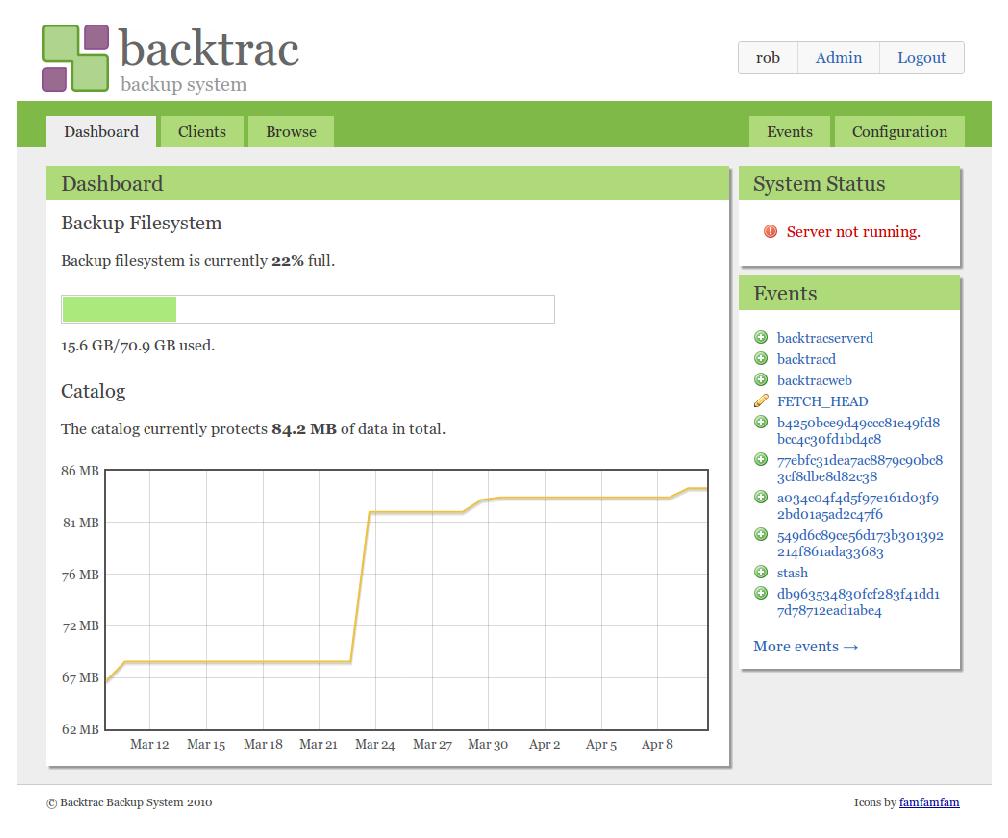
\includegraphics[width=\textwidth]{backtrac-dashboard}
    \end{center}
    \caption{A screenshot of the dashboard page}
    \label{fig:backtrac-dashboard}
\end{figure}

\subsection{Clients}
\label{sec:implementation-web-clients}

The clients interface allows the administrator to add, edit or delete backup
clients. When a client is added, it is configured with a secret key and a list
of paths to backup. Figure \ref{fig:backtrac-clients-add} shows a screenshot of
the form used when adding a client.

\begin{figure}[h]
    \begin{center}
        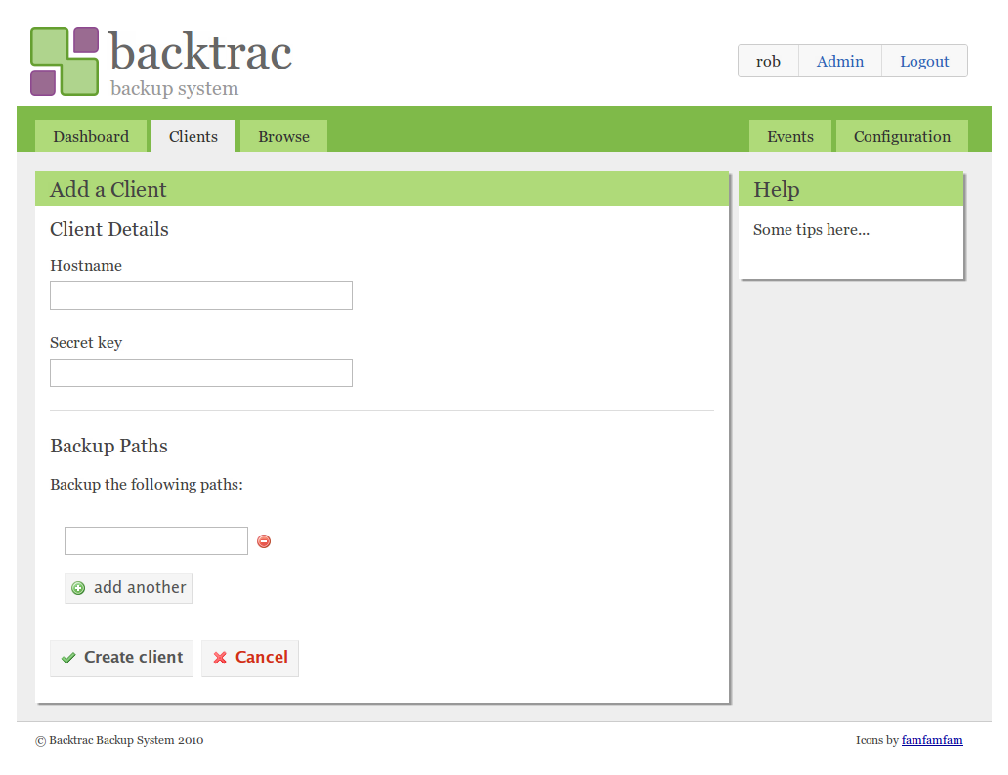
\includegraphics[width=\textwidth]{backtrac-clients-add}
    \end{center}
    \caption{A screenshot of the add client form}
    \label{fig:backtrac-clients-add}
\end{figure}

\subsection{Browse}
\label{sec:implementation-web-browse}

The administrator can browse the catalog of protected items through the web
interface, using the ``browse'' tab. The ``drill-down'' method is used to
provide a familiar way of traversing the filesystem once a client has been
chosen.

When browsing the catalog, the administrator can choose to show or hide deleted
files. A screenshot of the browsing interface is shown in figure
\ref{fig:backtrac-browse}.

\begin{figure}[h]
    \begin{center}
        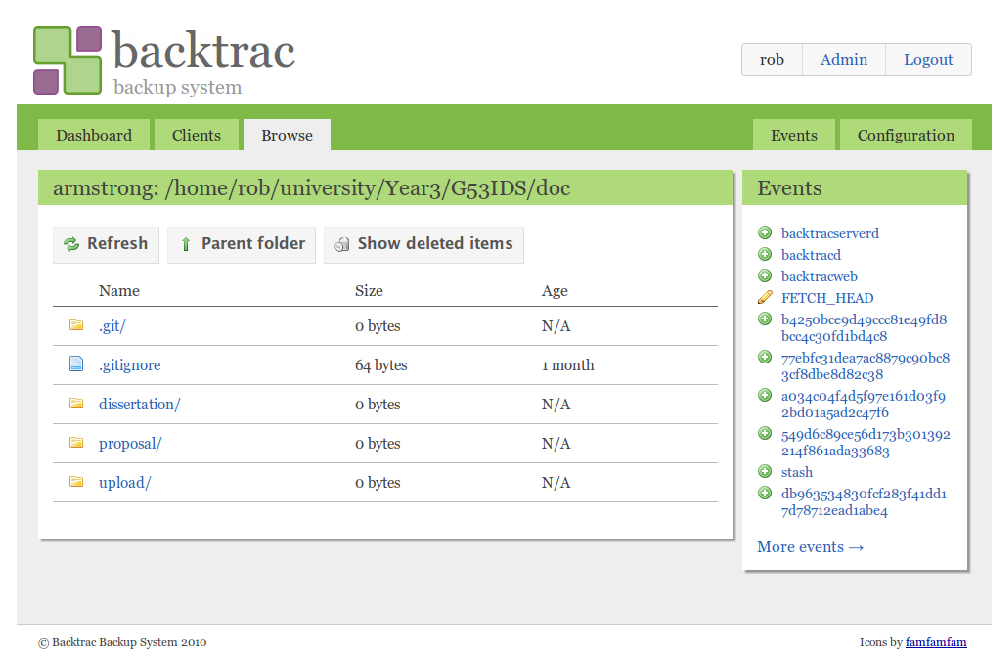
\includegraphics[width=\textwidth]{backtrac-browse}
    \end{center}
    \caption{A screenshot of the catalog browsing interface}
    \label{fig:backtrac-browse}
\end{figure}

Once a file has been selected, a detailed screen shows the different versions
of that file and their respective modification times and sizes. The
administrator can then choose to view one of the versions in the browser (in
the case of a plain text file, image or PDF document), download it, or restore
it to a chosen client. The selected version can be restored to the client from
which it originated, or any other client in the system. Also, it can either be
restored to its original location or another chosen path.

A screenshot of the detailed file view is shown in figure
\ref{fig:backtrac-file-detail}. As shown in the figure, a graph showing the
size of the file over time is also included on the file detail page---showing
how the file has evolved since it was first created.

\begin{figure}[h]
    \begin{center}
        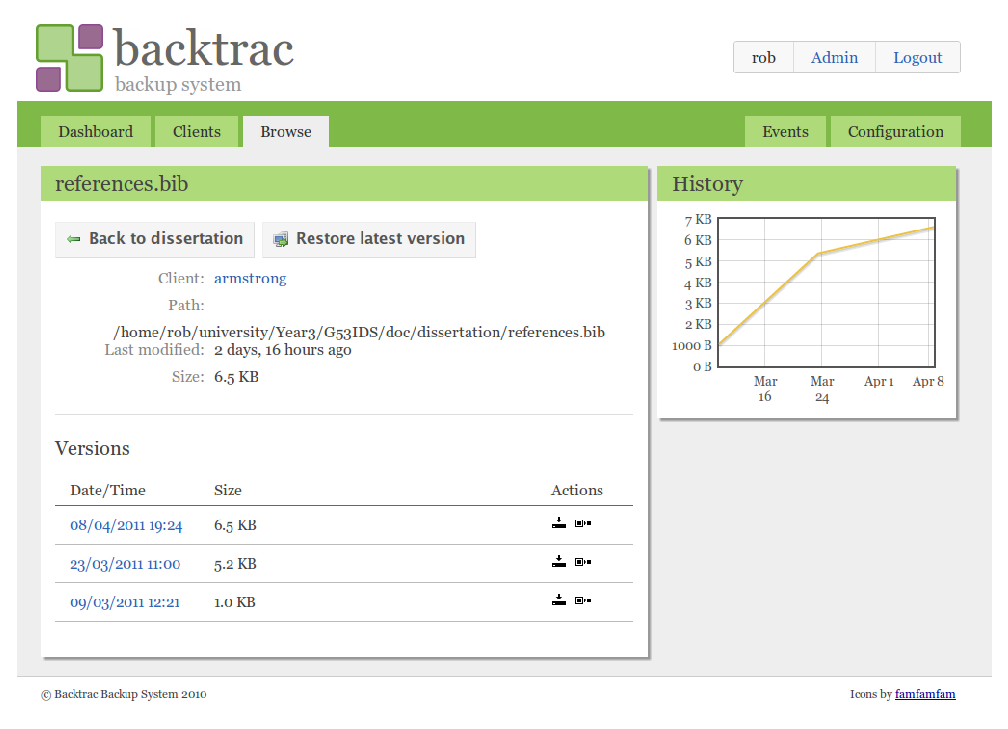
\includegraphics[width=\textwidth]{backtrac-file-detail}
    \end{center}
    \caption{A screenshot of the detailed file view}
    \label{fig:backtrac-file-detail}
\end{figure}

\subsection{Search}
\label{sec:implementation-web-search}

Search is widely considered to be something that is very difficult to get
right. Implementing search such that it returns relevant results in
a reasonable amount of time can be a time-consuming process.

Python has many libraries available which offer fast, tested search indexing.
\emph{Whoosh} is one such library, and is written in pure Python. This means
that is requires no code compilation, and is easy to install.

\begin{quote}
    \emph{Whoosh is a fast, featureful full-text indexing and searching library
    implemented in pure Python.}\footnote{http://www.whoosh.ca}
\end{quote}

Whoosh was used to implement the search functionality of the web interface in
this project, along with \emph{haystack}, the 3\textsuperscript{rd} party
search app for Django.

Haystack provides a Django-like API for searching data models, and can be
powered by a one of a number of backends. For this project, the Whoosh backend
was chosen due to the fact that it requires no additional dependencies or
compilation steps.

\section{Version Control}
\label{sec:implementation-versioncontrol}

Version control is an important aspect of any project, not only for retaining
the historical versioning information but also for centralising development in
one location. This also allows for up-to-date backups to be kept easily, and
prevents changes from being lost when developing on multiple workstations.

For this project, Git is used for version control with a central repository
stored on the GitHub web service.

\subsection{Distributed Version Control}

Distributed Version Control Systems (DVCS) are different to traditional Version
Control Systems in that there is no central ``authoritative'' repository
\cite{robert2006}. Instead, each developer ``clones'' the entire repository's
history onto their local development machine, and commits their changes back to
that local clone.

To share their changes, developers synchronise their repositories with each
user using a ``push'' and ``pull'' technique. With this approach, the
repositories are compared to find a common point in their history and then
merged together.

When using a DVCS, a central server can be used to store a repository which
everyone has access to, so that changes can be shared between all developers
effectively. There is, however, no tangible difference between the repository
stored on the server and those stored on the local machines. In effect, all
repositories are created equal. The only difference is that the server
containing the ``central'' repository is accessible reliably from the internet,
whereas a developer's machine may not be.

Though it may appear more complex than the traditional method of source control
(i.e. CVS or Subversion), it is fast becoming a very popular way of developing
software \cite{takhteyev2010}. It allows developers to participate in
open-source projects by ``forking'' the repository and applying their own
ideas, and then notifying the original author of their fork. The author may
then choose to merge the changes into the mainstream repository, directly
involving the developer in the project. Github \cite{Github} is the most
popular hosting system for Git, claiming to host over one million repositories
in 2010 \cite{takhteyev2010}.

This project's repository is hosted on GitHub, providing a centrally accessible
location for development. The project itself is released under the open-source
GNU General Public Licence version 3 (GPLv3) \cite{stallman1991}.
